\documentclass[11pt,oneside,twocolumn,openany,headings=optiontotoc,11pt,numbers=noenddot]{article}

\usepackage[a4paper]{geometry}
\usepackage[utf8]{inputenc}
\usepackage[T1]{fontenc}
\usepackage{lmodern}
\usepackage[ngerman]{babel}
\usepackage{ngerman}

\usepackage[onehalfspacing]{setspace}

\usepackage{fancyhdr}
\usepackage{fancybox}

\usepackage{rotating}
\usepackage{varwidth}

%Struktogramme
\usepackage[german,curves]{struktex}

\usepackage{pdflscape}
\usepackage{changepage}
\usepackage{graphicx}
\usepackage[bottom]{footmisc}
\usepackage{transparent}
\usepackage{graphbox}
\graphicspath{
	{Pics/PDFs/}
	{Pics/JPGs/}
	{Pics/PNGs/}
}
\usepackage{caption}
\usepackage{wrapfig}
\usepackage{marginnote}
\usepackage{tabularx}
\usepackage{dashrule}
\usepackage{soulutf8}
\usepackage{hhline}
%arydshln suppresses vertical lines in table
%\usepackage{arydshln}
\usepackage{multirow}
\usepackage{enumerate}
\usepackage[hidelinks]{hyperref}
\usepackage{listings}

\usepackage[table]{xcolor}
\usepackage{array}
\usepackage{enumitem,amssymb,amsmath}
\usepackage{interval}
\usepackage{cancel}
\usepackage{stmaryrd}
\usepackage{wasysym}
\usepackage{polynom}
\usepackage{diagbox}
\usepackage{dashrule}
\usepackage{framed}
\usepackage{mdframed}
\usepackage{karnaugh-map}
\usepackage{pdfpages}

\usepackage{blindtext}

\usepackage{eso-pic}

\usepackage{amssymb}
\usepackage{eurosym}

\usepackage[pages=some]{background}
\pagestyle{headings}
\renewcommand{\headrulewidth}{0.2pt}
\renewcommand{\footrulewidth}{0.2pt}
\newcommand*{\underdownarrow}[2]{\ensuremath{\underset{\overset{\Big\downarrow}{#2}}{#1}}}
\setlength{\fboxsep}{5pt}
\newcommand{\explainBelow}[3]{\underbrace{#1}_{\parbox{\widthof{#3}}{\footnotesize\raggedright #2}}}
\newcommand{\explainAbove}[3]{\overbrace{#1}^{\parbox{\widthof{#3}}{\footnotesize\raggedright #2}}}
\newcommand\footnoteref[1]{\protected@xdef\@thefnmark{\ref{#1}}\@footnotemark}


% Codestyle defined
\definecolor{codegreen}{rgb}{0,0.6,0}
\definecolor{codegray}{rgb}{0.5,0.5,0.5}
\definecolor{codepurple}{rgb}{0.58,0,0.82}
\definecolor{backcolour}{rgb}{0.95,0.95,0.92}
\definecolor{deepgreen}{rgb}{0,0.5,0}
\definecolor{darkblue}{rgb}{0,0,0.65}
\definecolor{mauve}{rgb}{0.40, 0.19,0.28}
\colorlet{exceptioncolour}{yellow!50!red}
\colorlet{commandcolour}{blue!60!black}
\colorlet{numpycolour}{blue!60!green}
\colorlet{specmethodcolour}{violet}

%Neue Spaltendefinition
\newcolumntype{L}[1]{>{\raggedright\let\newline\\\arraybackslash\hspace{0pt}}m{#1}}
\newcolumntype{M}{>{\centering\arraybackslash}X}
\newcommand{\cmnt}[1]{\ignorespaces}
%Textausrichtung ändern
\newcommand\tabrotate[1]{\rotatebox{90}{\raggedright#1\hspace{\tabcolsep}}}

%Intervall-Konfig
\intervalconfig {
	soft open fences
}

%Bash
\lstdefinestyle{BashInputStyle}{
	language=bash,
	basicstyle=\small\sffamily,
	backgroundcolor=\color{backcolour},
	columns=fullflexible,
	backgroundcolor=\color{backcolour},
	breaklines=true,
}
%Java
\lstdefinestyle{JavaInputStyle}{
	language=Java,
	backgroundcolor=\color{backcolour},
	aboveskip=1mm,
	belowskip=1mm,
	showstringspaces=false,
	columns=flexible,
	basicstyle={\footnotesize\ttfamily},
	numberstyle={\tiny},
	numbers=none,
	keywordstyle=\color{purple},,
	commentstyle=\color{deepgreen},
	stringstyle=\color{blue},
	emph={out},
	emphstyle=\color{darkblue},
	emph={[2]rand},
	emphstyle=[2]\color{specmethodcolour},
	breaklines=true,
	breakatwhitespace=true,
	tabsize=2,
}
%Python
\lstdefinestyle{PythonInputStyle}{
	language=Python,
	alsoletter={1234567890},
	aboveskip=1ex,
	basicstyle=\footnotesize,
	breaklines=true,
	breakatwhitespace= true,
	backgroundcolor=\color{backcolour},
	commentstyle=\color{red},
	otherkeywords={\ , \}, \{, \&,\|},
	emph={and,break,class,continue,def,yield,del,elif,else,%
		except,exec,finally,for,from,global,if,import,in,%
		lambda,not,or,pass,print,raise,return,try,while,assert},
	emphstyle=\color{exceptioncolour},
	emph={[2]True,False,None,min},
	emphstyle=[2]\color{specmethodcolour},
	emph={[3]object,type,isinstance,copy,deepcopy,zip,enumerate,reversed,list,len,dict,tuple,xrange,append,execfile,real,imag,reduce,str,repr},
	emphstyle=[3]\color{commandcolour},
	emph={[4]ode, fsolve, sqrt, exp, sin, cos, arccos, pi,  array, norm, solve, dot, arange, , isscalar, max, sum, flatten, shape, reshape, find, any, all, abs, plot, linspace, legend, quad, polyval,polyfit, hstack, concatenate,vstack,column_stack,empty,zeros,ones,rand,vander,grid,pcolor,eig,eigs,eigvals,svd,qr,tan,det,logspace,roll,mean,cumsum,cumprod,diff,vectorize,lstsq,cla,eye,xlabel,ylabel,squeeze},
	emphstyle=[4]\color{numpycolour},
	emph={[5]__init__,__add__,__mul__,__div__,__sub__,__call__,__getitem__,__setitem__,__eq__,__ne__,__nonzero__,__rmul__,__radd__,__repr__,__str__,__get__,__truediv__,__pow__,__name__,__future__,__all__},
	emphstyle=[5]\color{specmethodcolour},
	emph={[6]assert,range,yield},
	emphstyle=[6]\color{specmethodcolour}\bfseries,
	emph={[7]Exception,NameError,IndexError,SyntaxError,TypeError,ValueError,OverflowError,ZeroDivisionError,KeyboardInterrupt},
	emphstyle=[7]\color{specmethodcolour}\bfseries,
	emph={[8]taster,send,sendMail,capture,check,noMsg,go,move,switch,humTem,ventilate,buzz},
	emphstyle=[8]\color{blue},
	keywordstyle=\color{blue}\bfseries,
	rulecolor=\color{black!40},
	showstringspaces=false,
	stringstyle=\color{deepgreen}
}

\lstset{literate=%
	{Ö}{{\"O}}1
	{Ä}{{\"A}}1
	{Ü}{{\"U}}1
	{ß}{{\ss}}1
	{ü}{{\"u}}1
	{ä}{{\"a}}1
	{ö}{{\"o}}1
}

% Neue Klassenarbeits-Umgebung
\newenvironment{worksheet}[3]
% Begin-Bereich
{
	\newpage
	\sffamily
	\setcounter{page}{1}
	\ClearShipoutPicture
	\AddToShipoutPicture{
		\put(55,761){{
				\mbox{\parbox{385\unitlength}{\tiny \color{codegray}BBS I Mainz, #1 \newline #2
						\newline #3
					}
				}
			}
		}
		\put(455,761){{
				\mbox{\hspace{0.3cm}
\includegraphics[width=0.2\textwidth]{../../logo.pdf}}
			}
		}
	}
}
% End-Bereich
{
	\clearpage
	\ClearShipoutPicture
}

\setlength{\columnsep}{3em}
\setlength{\columnseprule}{0.5pt}

\pagestyle{empty}

\geometry{left=1.50cm,right=1.50cm,top=2.50cm,bottom=1.00cm,includeheadfoot}

\begin{document}
	\begin{worksheet}{BS EGSIE 18}{1. Lehrjahr, LF 4 - Informationstechnische Systeme bereitstellen}{Verarbeitungsgeräte - Externe Schnittstellen}
		\onehalfspacing
		\subsection*{PS/2}
		Üblicherweise werden hier Tastatur und Maus angeschlossen. Die angeschlossenen Peripheriegeräte können direkt nach dem Computerstart genutzt werden.\\
		Die Anschlüsse sind baugleich, unterscheiden sich aber in ihrer Funktion. Um die Zuordnung zu erleichtern, werden die Stecker an den Geräten in der zugehörigen Farbe produziert.\\
		Üblicherweise ist der Mausanschluss (grün) oben und der für die Tastatur (lila) unten.
		\subsection*{Parallel (IEEE 1284, Centronics oder LPT-Anschluss)}
		Wird für eine schnelle Datenübertragung genutzt, da hier 8 Bit gleichzeitig (parallel) übertragen werden können.\\
		Häufige Anwendungsbereiche sind Drucker (LPT = \textbf{L}ine\textbf{P}rin\textbf{t}er), Scanner aber auch externe Laufwerke. Ein Datenaustausch zwischen zwei Computern ist aber auch möglich.\\
		\footnotesize{Abgelöst wurde der Parallelanschluss vor geraumer Zeit von USB.}\normalsize
		\subsection*{Seriell (RS-232C oder COM)}
		Bei der Datenübertragung werden die Daten schrittweise (seriell), also nacheinander übertragen, sodass hiermit nur eine geringe Übertragungsgeschwindigkeit erreicht werden kann.\\
		Vorteilhaft hingegen ist, dass die Übertragung weniger störanfällig ist, wodurch auch eine Übertragung über 1000 Meter hinweg möglich ist.\\
		Wie auch bei der Parallelschnittstelle ist ein Datenaustausch zwischen zwei Computern möglich.\\
		\footnotesize{Abgelöst wurde die serielle Schnittstelle von USB, sodass der serielle Anschluss bei neueren Computern nicht mehr zu finden ist.}\normalsize
		\subsection*{USB - Universal Serial Bus}
		An USB können bis zu 127 Geräte gleichzeitig angeschlossen werden. Die angeschlossenen Geräte werden in der Regel bei allen aktuell verwendeten Betriebssystemen automatisch erkannt und notwendigen Programme werden automatisch installiert.\\
		Mittlerweile kann eine Vielzahl von Geräten per USB mit dem Computer verbunden werden. Er hat sich zu einem der wichtigsten Anschlusstypen entwickelt.\\
		\par\noindent
		Bei den Anschlüssen ist zu beachten, dass es hier marginale Unterschiede gibt.\\
		\begin{tabularx}{0.48\textwidth}{MMM}
			USB 1.1 - bis zu 12 Mbit/s & USB 2.0 - bis zu 480 Mbit/s & USB 3.0 - bis zu 640 Mbit/s
		\end{tabularx}
		\subsection*{Netzwerk (RJ-45)}
		Ermöglicht eine Verbindung zu einem kabelgebundenen Netzwerk. Abhängig vom Einsatzgebiet können Übertragungsgeschwindigkeiten von 10MBit/s bis hin zu 10GBit/s erreicht werden.
		\subsection*{Sound, analog}
		Der Onboard-Soundchip kann von der Funktionalität mit einer klassischen Hi-Fi-Anlage verglichen werden. Den verschiedenen 3,5''-(Stereo)-Klinkenstecker-Anschlüssen kommen unterschiedliche Funktionen zu:
		\begin{itemize}
			\item Blau: Eingang Stereo (MP3-Player, Hi-Fi-Anlage)
			\item Grün: Ausgang Stereo (Lautsprecher vorne, Kopfhörer)
			\item Rot/Rosa: Eingang Mono (Mikrofon)
			\item Grau/Silber: Ausgang Stereo (Lautsprecher Seite)
			\item Schwarz: Ausgang Stereo (Lautsprecher hinten)
			\item Orange: Ausgang Center-Lautsprecher und Subwoofer
		\end{itemize}
		\subsection*{Sound, digital}
		Die Soundsignale werden bereits digital an die Buchse geleitet, so dass ein Digital-Analog-Wandler (auf der Soundkarte bzw. im Soundchip) nicht nötig ist.\\
		Die Umwandlung geschieht in der optisch oder koaxial angeschlossenen Hi-Fi- bzw. Surround-Anlage.
		\subsection*{Monitor, analog (VGA - Video Graphics Array)}
		Beim anschluss eines TFT-Display über den VGA-Anschluss werden die übetragenen Bildsignale digital/analog bzw. analog/digital umgewandelt, so dass erhebliche Einbußen bei der Bildqualität auftreten.\\
		\footnotesize{Aufgrund der Digitalisierung wird diese Schnittstelle in naher Zukunft keine Relevanz mehr haben.}\normalsize
		\subsection*{Monitor, digital (DVI - Digital Visual Interface)}
		Moderne Bildschirme benötigen digitale Signale, welche durch diese und die nachfolgenden Schnittstellen bereitgestellt werden.\\
		Die Datenübertragung erfolgt verlustfrei und ermöglicht zudem eine bessere Bildqualität als der analoge Anschluss.\\
		Auflösungen bis zu 2560 x 2048 Pixel sind mit entsprechenden Kabeln möglich.\\
		\footnotesize{DVI wird immer mehr durch HDMI, DisplayPort oder Thunderbolt ersetzt.}\normalsize
		\subsection*{Monitor, digital (HDMI - High Defintion Multimedia Interface)}
		Wird als Nachfolger von DVI gehandelt, da er zusätzlich noch über Audioübertragung und einen Kopierschutz (HDCP) verfügt. Hierdurch können HD-Inhalte auf Bildschirmen mit einer Auflösung von bis zu 4096 x 2160 Pixeln ermöglicht.
		\subsection*{Monitor, digital (Displayport)}
		Ermöglicht eine Bildschirmauflösung von bis zu 3840 x 2160 Pixeln und kann auch 3D-Inhalte verarbeiten.
		\subsection*{FireWire}
		Gilt als serielle Hochgeschwindigkeitsschnittstelle, welche vor allem im Video- und Audiobereich eingesetzt wird. Es existieren aber auch externe Festplatten mit einem FireWire-Anschluss.\\
		Ähnlich zu USB können FireWire-Geräte an den laufenden Computer angeschlossen und direkt verwendet werden.\\
		Trotz der hohen Übertragungsgeschwindigkeiten von 800, 1600 und 3200 MBit/s konnte sich diese Schnittstelle nicht durchsetzen.\\
		\footnotesize{USB-Anschlüsse werden als kostengünstigere Alternative verwendet und konnten sich auf die Dauer durchsetzen.}
		\subsection*{eSATA}
		Die standardmäßigen an die interne SATA angeschlossenen Festplatten bzw. BD/DVD/CD-R/W-Laufwerke werden über eSATA an das PC-Gehäuse geführt.\\
		Hauptsächlich wird dieser Anschluss für externe Festplatten verwendet. 
		\subsection*{Weitere optionale externe Schnittstellen an der Vorderseite des Gehäuses}
		Häufig finden sich an modernen Computern an der Vorder- oder Oberseite des Computers verschiedene zusätzliche externe Anschlüsse. Hier stehen häufig neben weiteren Audio- und USB-Anschlüssen noch Speicherkartenleser zur Verfügung.\\
		\par\noindent
		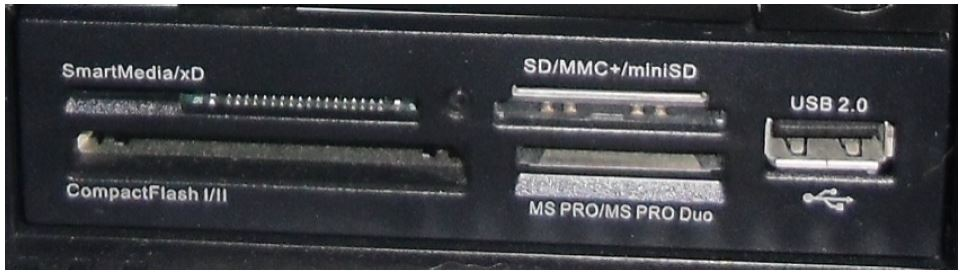
\includegraphics[width=0.48\textwidth]{../99_Bilder/SD.jpg}
	\end{worksheet}
\end{document}